\documentclass[24pt, letterpaper]{article}
\usepackage[utf8]{inputenc}
\usepackage{graphicx}
\usepackage{placeins}
\graphicspath{{images/}}

% document date time and such
\title{Lab 1}
\author{Michael Trey Peterson}
\date{02/15/2022}

% document meat and potatoes
\begin{document}
\maketitle
\tableofcontents
	\section{Creating Tensors}
		\begin{figure}[ht]
			\centering
			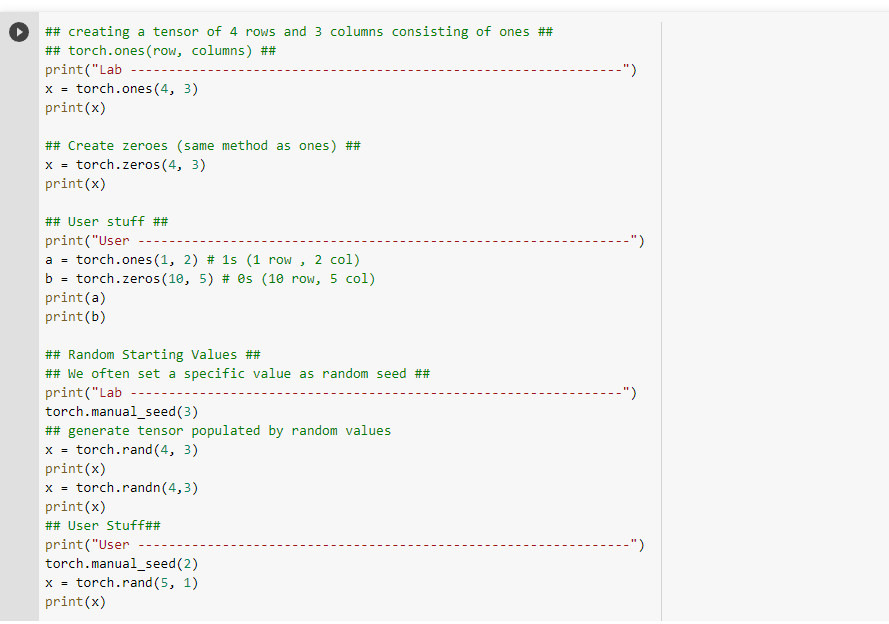
\includegraphics[width=0.7\linewidth]{Lab1Img/CTensor_Code}
			\caption{Tensor Creation Code}
			\label{fig:ctensorcode}
		\end{figure}
		\begin{figure}[ht]
			\centering
			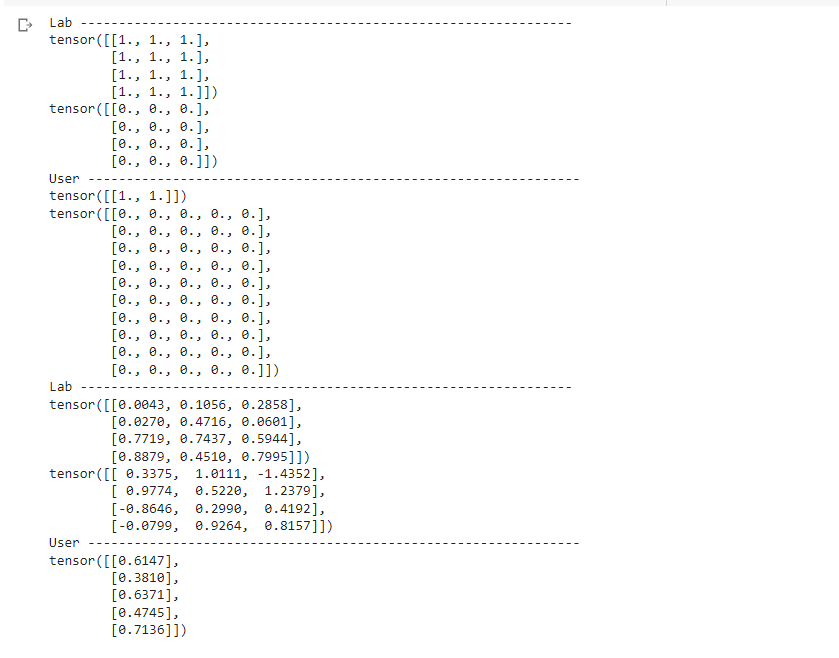
\includegraphics[width=0.7\linewidth]{Lab1Img/CTensor_Result}
			\caption{Tensor Creation Output}
			\label{fig:ctensorresult}
		\end{figure}			
		\FloatBarrier
		
	\section{Tensor Operations}
		\begin{figure}[ht]
			\centering
			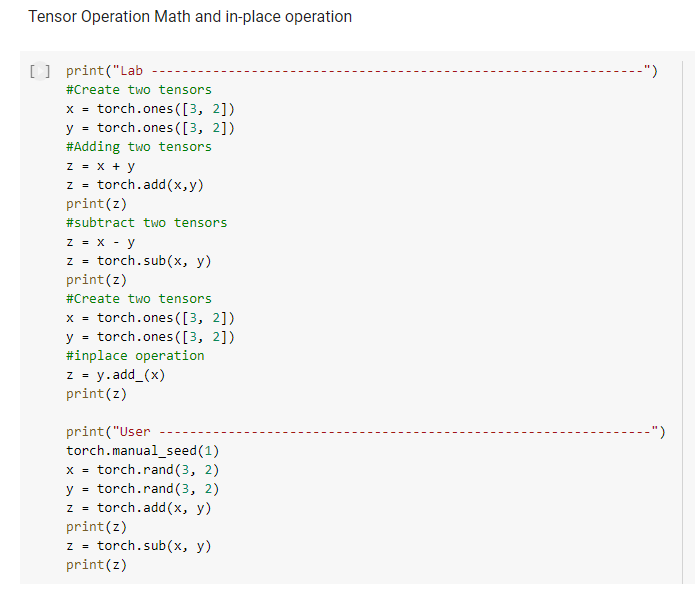
\includegraphics[width=0.7\linewidth]{Lab1Img/TensorOperation_Code}
			\caption{Tensor Operation Code}
			\label{fig:tensoroperationcode}
		\end{figure}
		\begin{figure}[ht]
			\centering
			\includegraphics[width=0.7\linewidth]{Lab1Img/TensorOperation_result}
			\caption{Tensor Operation Output}
			\label{fig:tensoroperationresult}
		\end{figure}	
		\begin{figure}
			\centering
			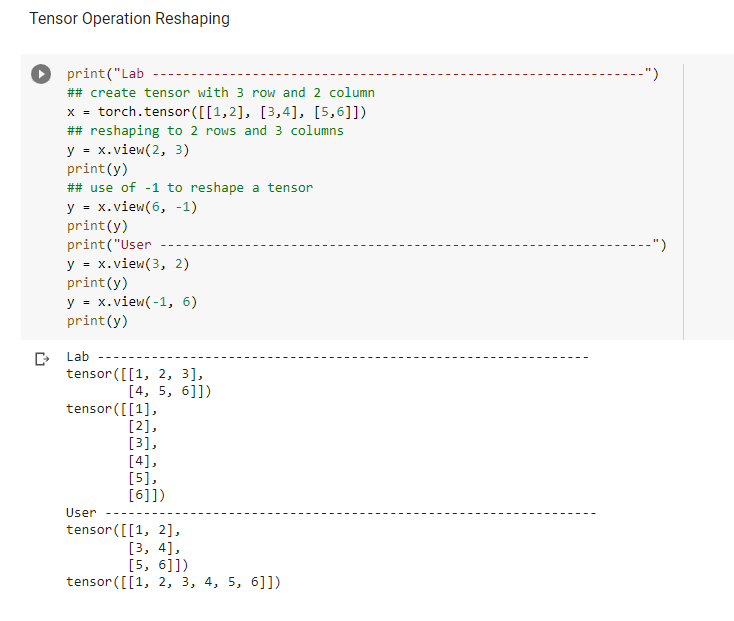
\includegraphics[width=0.7\linewidth]{Lab1Img/TensorReshaping}
			\caption{Tensor Reshaping}
			\label{fig:tensorreshaping}
		\end{figure}
		\begin{figure}
			\centering
			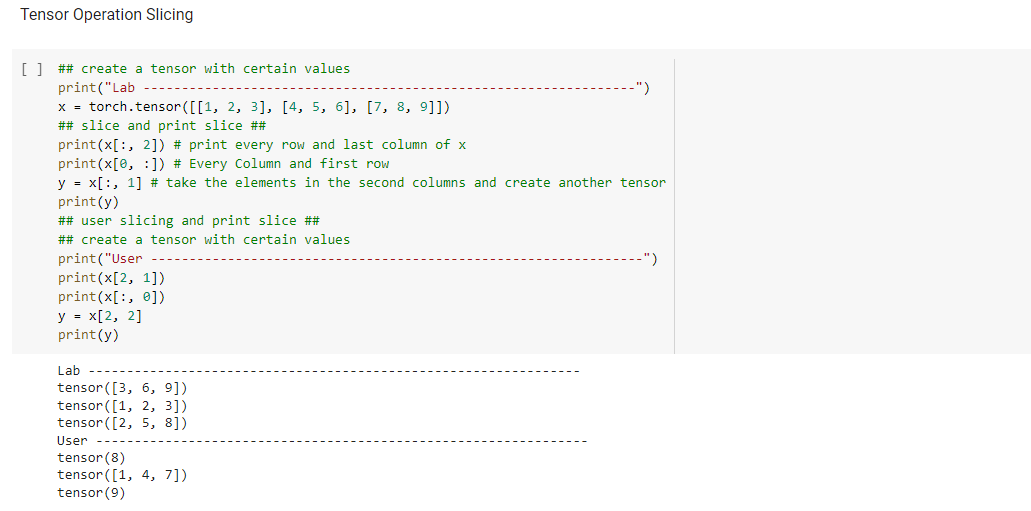
\includegraphics[width=0.7\linewidth]{Lab1Img/TensorSlicing}
			\caption{Tensor Slicing}
			\label{fig:tensorslicing}
		\end{figure}
		% holy fuck this works	
		\FloatBarrier
		
	\section{CUDA + autograd}
		\begin{figure}[ht]
			\centering
			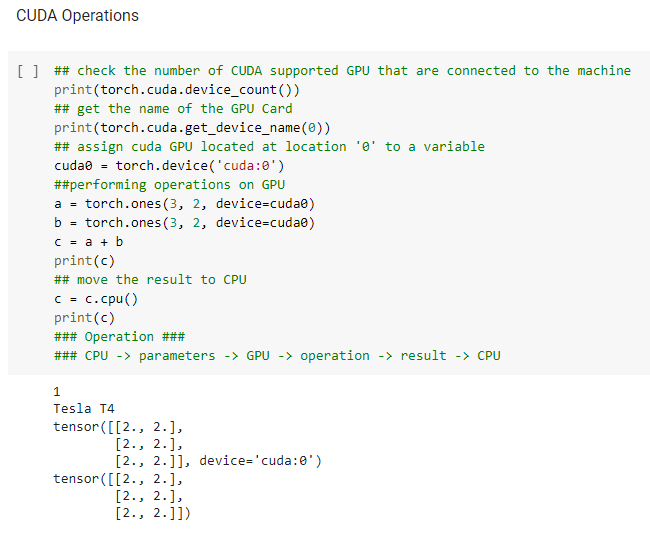
\includegraphics[width=0.7\linewidth]{Lab1Img/CUDA}
			\caption{CUDA Code}
			\label{fig:CUDA}
		\end{figure}
		\begin{figure}[ht]
			\centering
			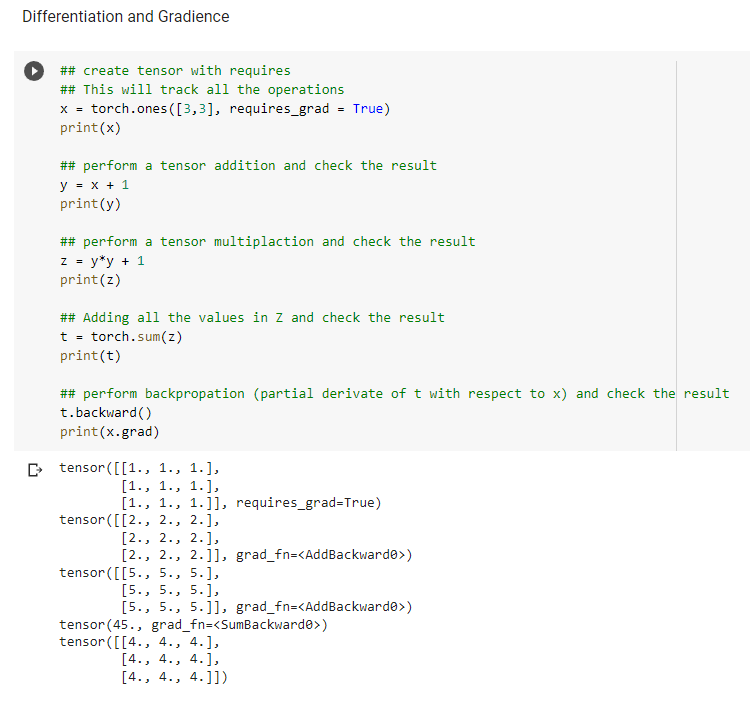
\includegraphics[width=0.7\linewidth]{Lab1Img/Gradience}
			\caption{Gradience code}
			\label{fig:gradience}
		\end{figure}
		% holy fuck this works		
		\FloatBarrier			
	
	\section{Toy Example}
	The following shows code made to train a linear model in 4 iterations. The linear model consists of the toy example presented in the lab as a way to make sure the model is functioning correctly (results are cross-referenced with lecture). The model takes an input and weight tensor of size n and then performs a dot product, the product is alias'd as z and the sum is alias'd as t. Since the model is linear an activation function isn't needed. To perform training the error is found by taking the target - result, error, and then multiplying the error by the learning rate and input (with it's corresponding weight) to give a delta weight. The delta weight is then added to the original weight.
		\begin{figure}[hb!]
			\centering
			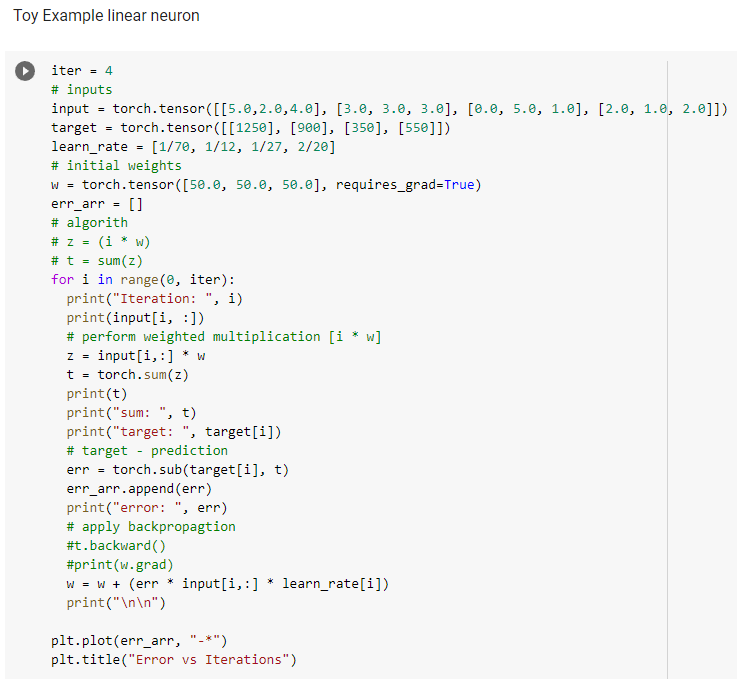
\includegraphics[width=0.7\linewidth]{Lab1Img/Linear_Code}
			\caption{Linear Neuron Code}
			\label{fig:Linear Code}
		\end{figure}
		\FloatBarrier	
	As shown the results correspond with the toy example slides to demonstrate successful training of the linear model.
		\begin{figure}[ht]
			\centering
			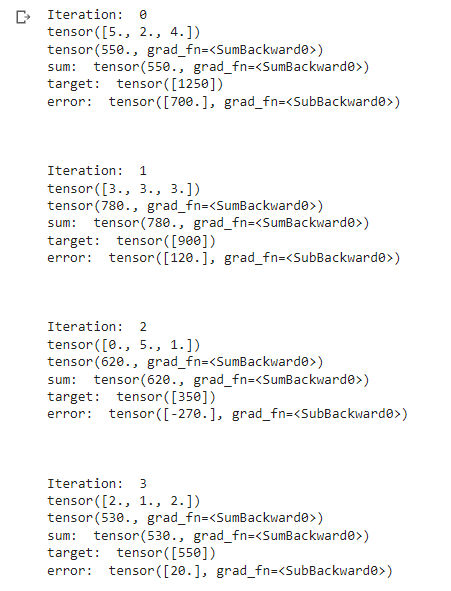
\includegraphics[width=0.7\linewidth]{Lab1Img/Linear_R1}
			\caption{Gradience Result}
			\label{fig:Linear Result}
		\end{figure}
		\FloatBarrier	
	A visual representation of the errorr shows convergence to 0 meaning that the model is training and the input/target have a realizable pattern.
		\begin{figure}[ht]
			\centering
			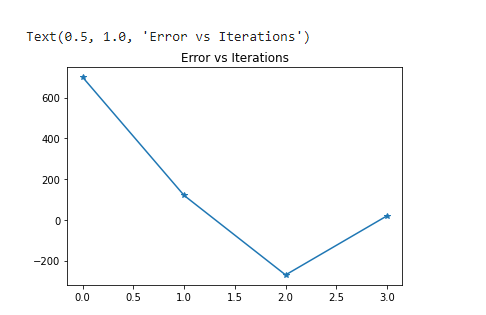
\includegraphics[width=0.7\linewidth]{Lab1Img/Linear_R2}
			\caption{Error Graph}
			\label{fig:Linear Result}
		\end{figure}
		% holy fuck this works		
		\FloatBarrier	
	
	

% This line here is a comment. It will not be printed in the document.
\end{document}